\documentclass{article}
\usepackage{amsmath}
\usepackage{graphicx}
\graphicspath{ {./images} }
\usepackage{float}

\setlength{\parindent}{0pt}
\hbadness=10000

\title{MP 2.2 Design Document}
\author{Kevin Zhang}
\date{\today}

\begin{document}

\maketitle

\section{Overview}

In this MP, we explore how explore two new concepts: using RabbitMQ to asynchronously replicate state across multiple clusters and replicating state between master and slave servers. Replicating the state of the SNS has many benefits, include fault tolerance (if a master server goes down, the slave can take over), increase load tolerance, and reduce latency among others.

\section{Client}

The client functionality remains the same as MP 2.1. From the client's perspective, nothing about the system has changed, which is described as "distribution transparency."

\section{Master/Slave Servers}

To accomplish master/slave replication, each SNS server is now replicated to form a master/slave pair. For this MP, we assume each cluster has up to 2 servers (one master, one slave).\\

Only master servers interact with clients and do so via synchronous RPCs. If a slave server exists on the cluster, the master forwards all user requests to the slave; thus, from the slave's perspective, the master looks like a client. As an implementation detail, I configured my SNS servers to lazily check whether they are a master server upon each client request.\\

To assign server roles, we go by order of registration. The first server on a cluster that registers with the coordinator is given the master role. Any subsequent servers that register on the same cluster become slaves.\\

For this MP, I updated the core logic of my SNS servers. All user info is persisted in the filesystem: each user has ``user\_timeline.txt," ``user\_following.txt," and ``user\_followers.txt" files that store information about the user's timeline posts, users they follow, and users that follow them, respectively. In addition, each server has an "all\_users.txt" file that records the existence of all users currently logged into the SNS.\\

There also exists an in-memory cache on each server that caches information from the filesystem, providing quick access to the user list and each user's followers. This in-memory cache is frequently updated by a background thread that reads each user's files from the filesystem (every 5 seconds).\\

Like before, each server has a background thread responsible for sending heartbeats to the coordinator. The first heartbeat registers the server with the coordinator, and subsequent heartbeats maintain the server's "alive" status.\\

Whenever a master server fails (the coordinator misses 2 consecutive heartbeats), a new server on its cluster (if exists) is appointed as a master. This process is done lazily: the new master does not know it is a master until it serves its next client request. As discussed earlier, an SNS server only discovers whether it is a master before returning from a client RPC.\\

\section{Coordinator}

The coordinator now maintains a table of follower synchronizer processes alongside its routing table of servers. Similar to the routing table, this synchronizer table is broken down by cluster; synchronizer processes are assigned to a cluster by the formula $(\text{synchronizerID} - 1) \bmod 3 + 1$, which is the same formula used to assign a client to a cluster.\\

Follower synchronizers are assigned to SNS servers by order of registration. For example, the follower synchronizer that's registered first is assigned to the SNS server that was assigned first, and so on.\\

The coordinator has a background thread that checks for heartbeats from all registered servers every 5 seconds. If a server or synchronizer misses 2 consecutive heartbeats (10 seconds), it is declared as dead. If the server was a master for its cluster, then the slave will be promoted with the logic explained in the \textbf{Master/Slave Servers} section.\\

Otherwise, the coordinator remains the same as before.\\

\section{Follower Synchronizer}

A follower synchronizer is a process that's responsible for publishing the local server's state, making it available for other servers, including servers in other clusters. The intent is for all servers on all clusters to eventually converge to the same state (in their filesystem):

\begin{itemize}
	\item ``all\_users.txt" should be the same across all servers
	\item All user's followers should be the same across all servers. A file that contains ``following" information is not strictly necessary.
	\item The timeline files of a user should be updated if someone they follower makes a post, even if the two users are not on the same server/cluster.
	\item The state of a master and slave on the same cluster should be exactly the same
\end{itemize}

To achieve this synchronization, the follower synchronizers use RabbitMQ, a message broker library, to asynchronously publish the server's state. We use a publish-subscribe messaging model: each synchronizer has a producer whose sole purpose is to publish messages to RabbitMQ and a consumer whose sole purpose is to consume messages delivered from RabbitMQ and apply changes accordingly. This model allows us to synchronize server state in the background without affecting the SNS client's time-senstivie synchronous RPCs.\\

In terms of implementation details, I perform all messaging via RabbitMQ exchanges. Exchanges act as middlemen that can forward any messages they receive to any consumers attached to the exxchange. This allows a producer to easily broadcast a message to any interested parties.

Each synchronizer declares 3 exchanges: ``all\_users," ``relations," and ``timelines" that are each responsible for a specific type of message. For example, any message regarding user relationships is sent to the ``relations" exchange, which is then forwarded to any consumer that has subscribed to messages from that exchange.

\section{Test Cases}

\begin{figure}[H]
	\centering
	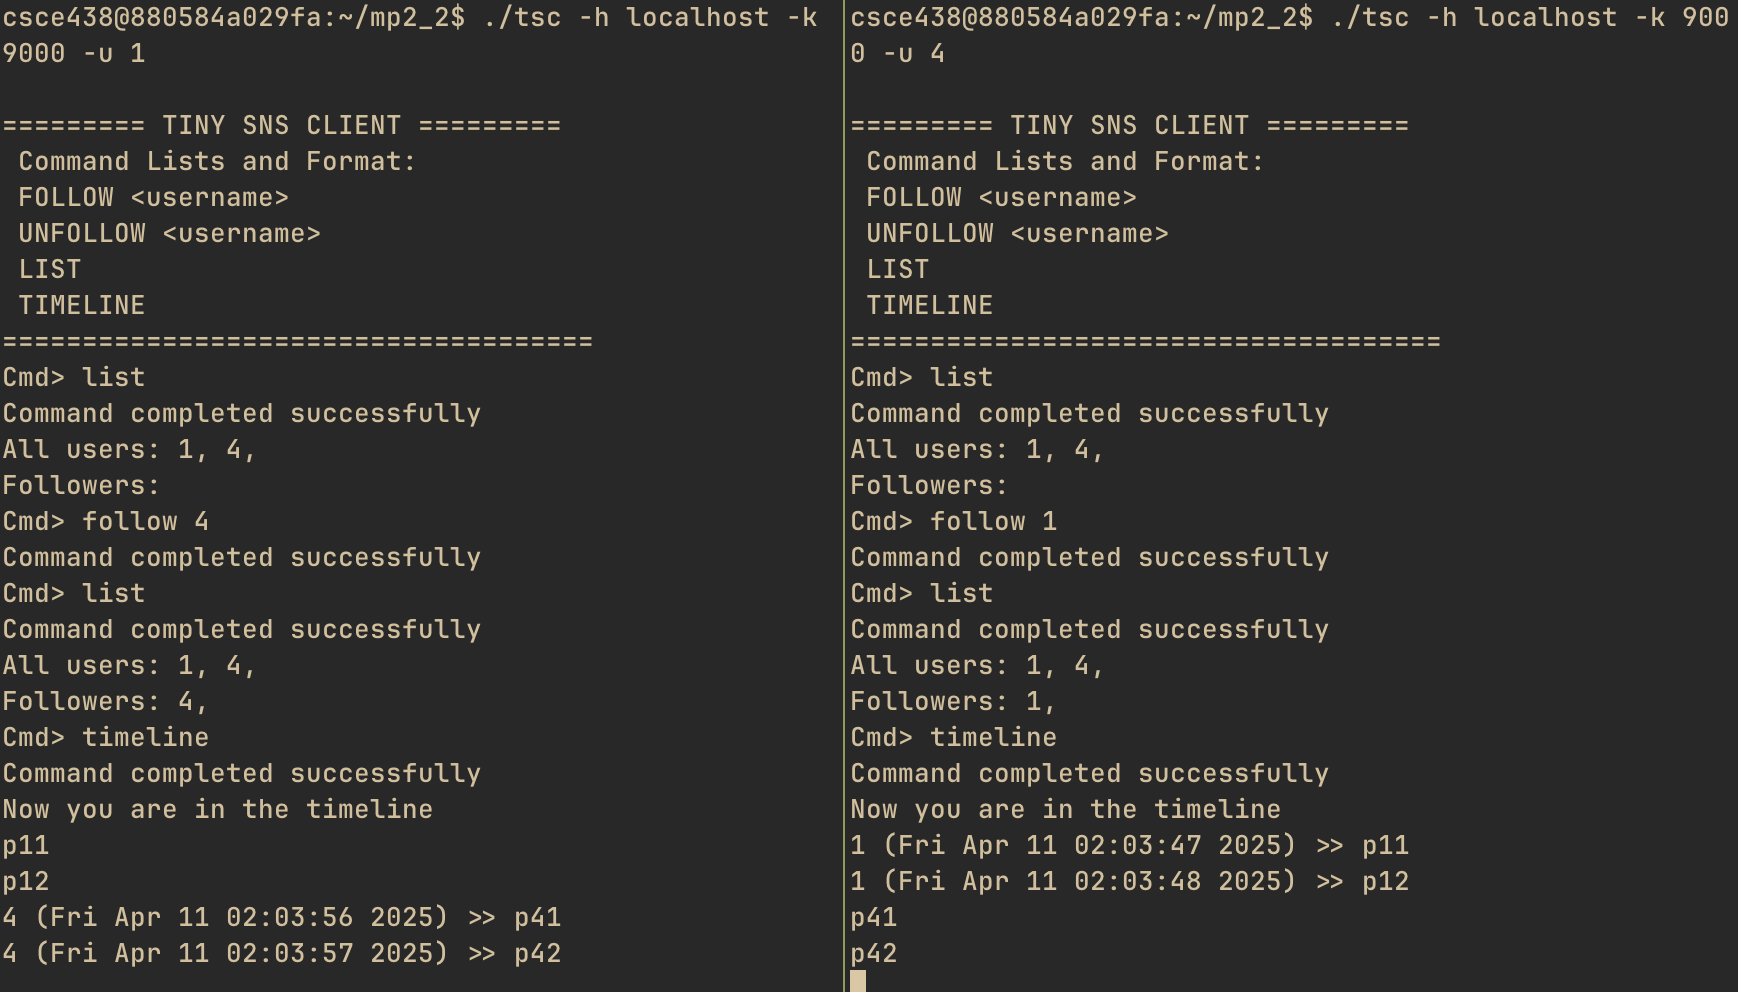
\includegraphics[width=\textwidth]{test1.png}
	\caption{sanity check}
\end{figure}

\begin{figure}[H]
	\centering
	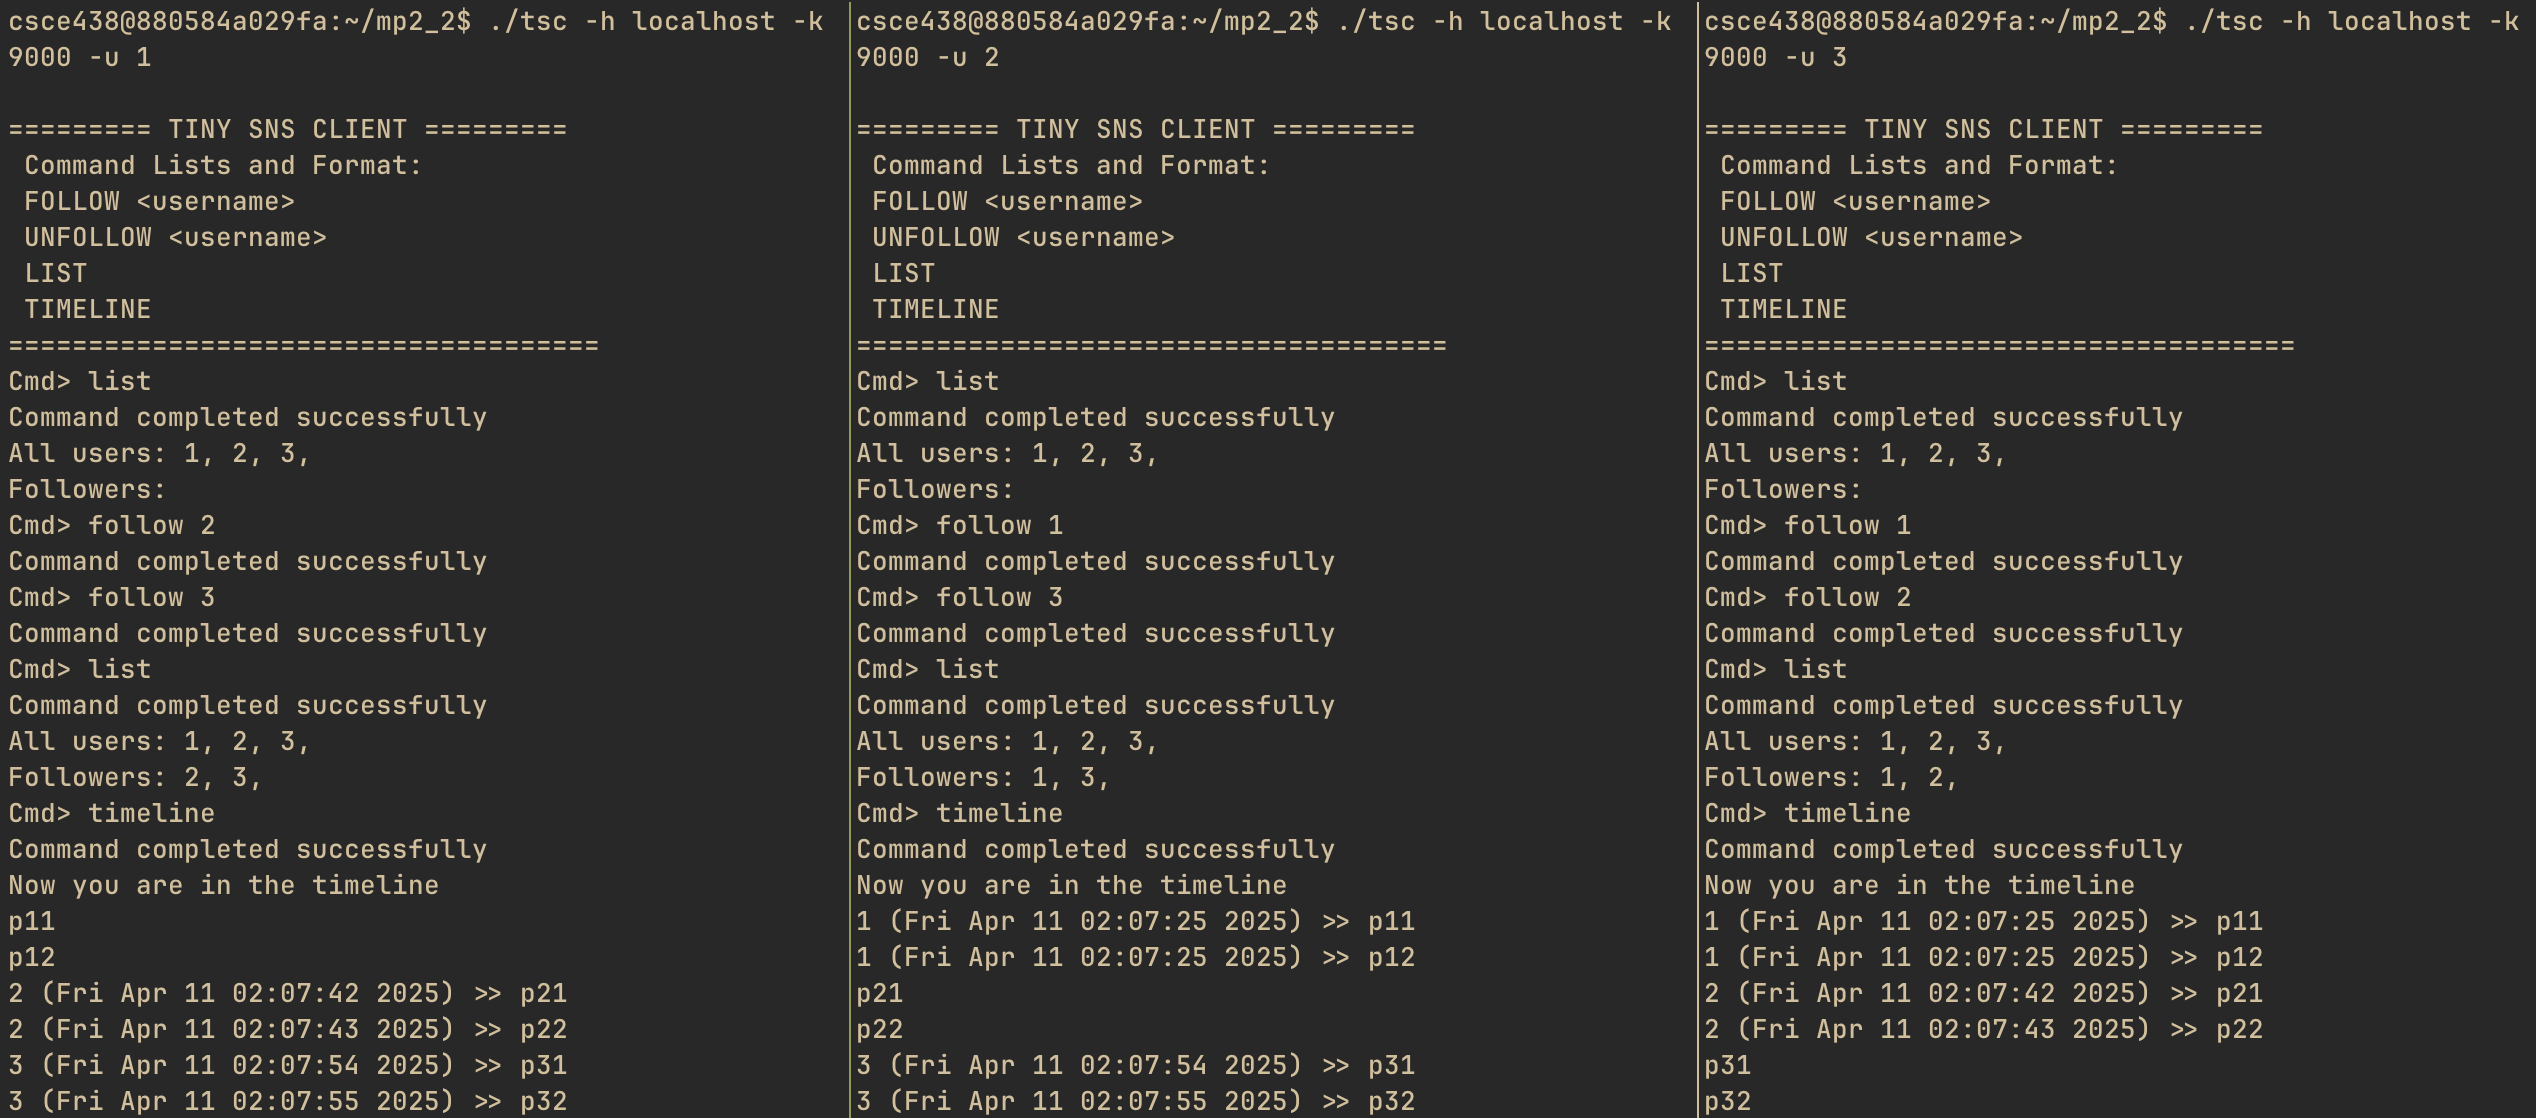
\includegraphics[width=\textwidth]{test2.png}
	\caption{testing multiple servers}
\end{figure}

\begin{figure}[H]
	\centering
	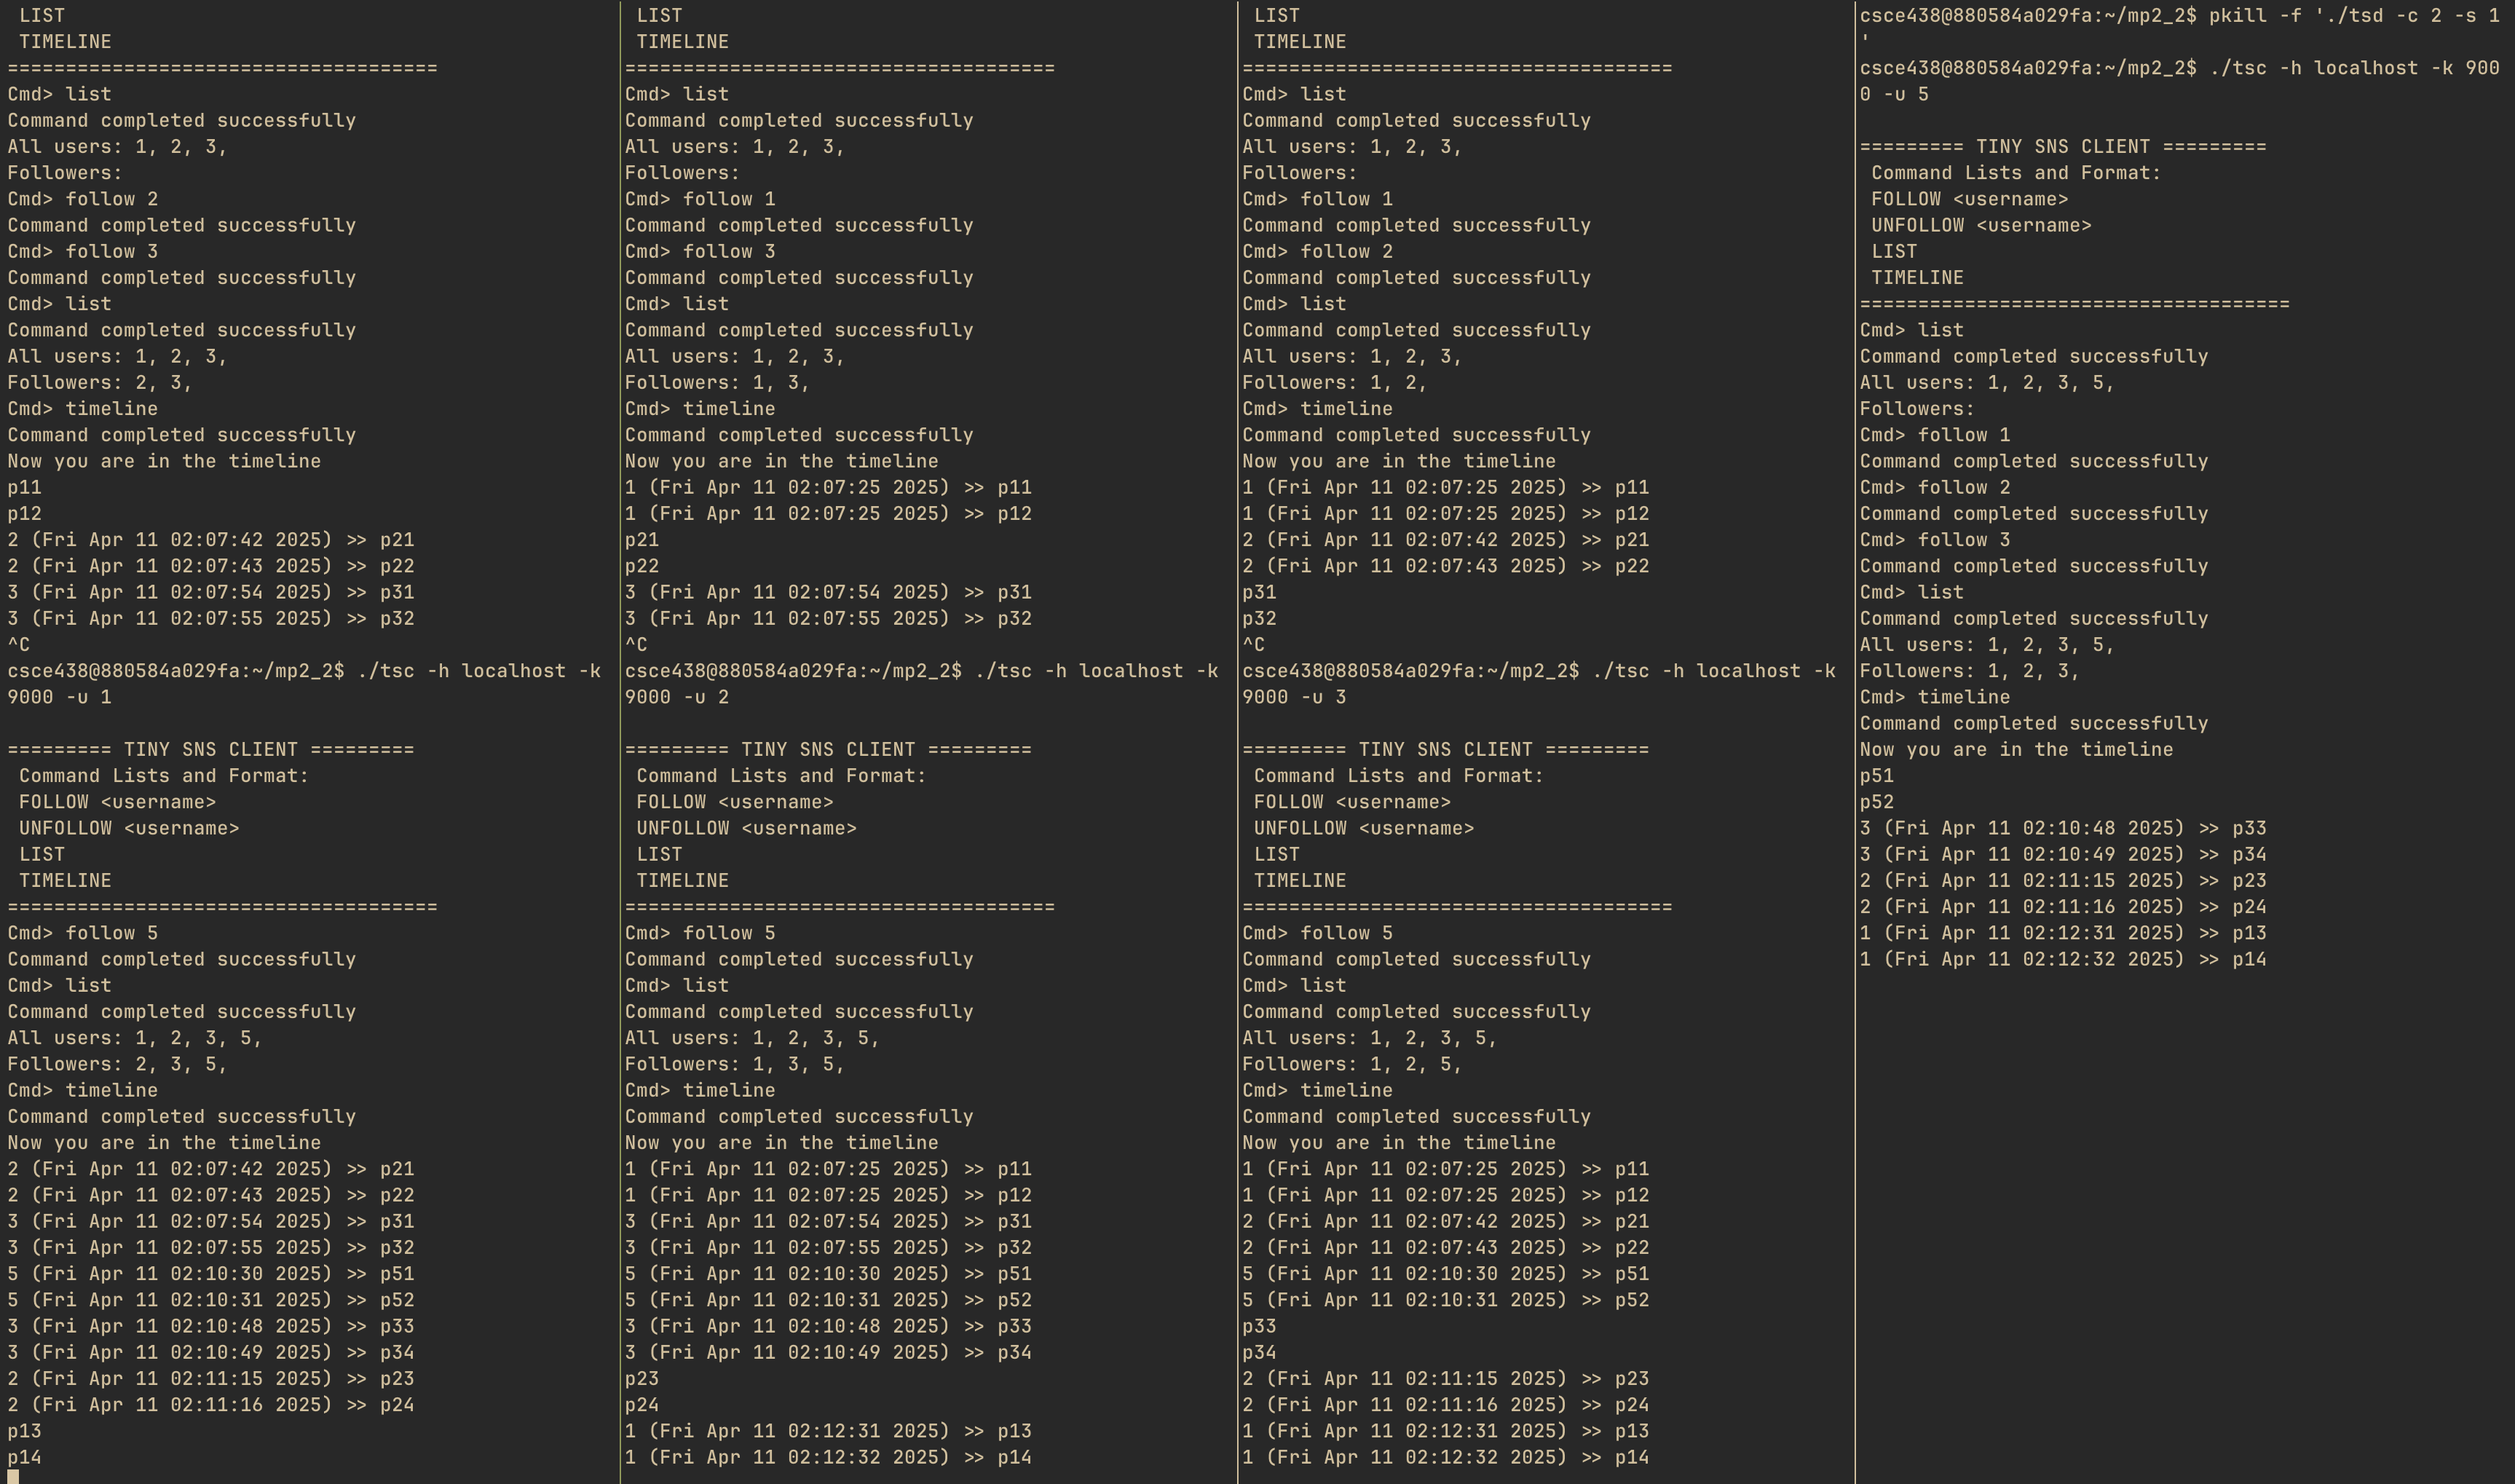
\includegraphics[width=\textwidth]{test3.png}
	\caption{testing resilience}
\end{figure}

\end{document}
